% ------------------------------------------------------------------------------
% TYPO3 Version 10.3 - What's New (German Version)
%
% @license	Creative Commons BY-NC-SA 3.0
% @link		https://typo3.org/help/documentation/whats-new/
% @language	German
% ------------------------------------------------------------------------------

\section{Einführung}
\begin{frame}[fragile]
	\frametitle{Einführung}

	\begin{center}\huge{Einführung}\end{center}
	\begin{center}\huge{\color{typo3darkgrey}\textbf{Fakten}}\end{center}

\end{frame}

% ------------------------------------------------------------------------------
% TYPO3 Version 10.3 - The Facts

\begin{frame}[fragile]
	\frametitle{Einführung}
	\framesubtitle{TYPO3 Version 10.3 - Fakten}

	\begin{itemize}
		\item Veröffentlichungsdatum: 25. Februar 2020
		\item Releasetyp: Sprint Release
	\end{itemize}

	\begin{figure}
		
\includegraphics[width=0.95\linewidth]{Introduction/typo3-v10-3-banner.png}
	\end{figure}

\end{frame}

% ------------------------------------------------------------------------------
% TYPO3 Version 10.3 - Executive Summary

\begin{frame}[fragile]
	\frametitle{Einführung}
	\framesubtitle{Zusammenfassung}

	\small
		Als letzte Sprint-Version des v10-Zyklus ist TYPO3 Version 10.3 die so genannte
		"\href{https://typo3.org/article/land-ho-feature-freeze-ahead}{Feature Freeze}"
		-Version. Das bedeutet, dass von nun an bis zur LTS-Veröffentlichung im April
		keine neuen Funktionen mehr hinzugefügt werden. Das Core-Team und alle Mitwirkenden konzentrieren sich auf das Testen, Polieren und Verfeinern der Freigabe.

		\vspace{0.2cm}

		Es gibt jedoch einige Ausnahmen für kleinere Verbesserungen zur Vervollständigung von Funktionen, die
		bereits in früheren v10-Sprint-Versionen hinzugefügt wurden.

		\vspace{0.2cm}

		Wenn Sie ein Erweiterungsentwickler sind, veröffentlichen Sie bitte v10-kompatible Versionen Ihrer 
		Erweiterungen. Dies wird es der TYPO3-Community erleichtern, TYPO3 v10 zu übernehmen, sobald die
		LTS-Version veröffentlicht wird.

		\vspace{0.2cm}

		Ein letzter wichtiger Punkt: Vergessen Sie nicht, an einer
		\href{https://typo3.org/community/events/v10-parties}{Release-Party} teilzunehmen oder selbst eine
		zu organisieren!

	\normalsize

\end{frame}

% ------------------------------------------------------------------------------
% System Requirements

\begin{frame}[fragile]
	\frametitle{Einführung}
	\framesubtitle{Systemvoraussetzungen}

	\begin{itemize}
		\item PHP Version 7.2, 7.3 oder 7.4
		\item PHP Einstellungen:

			\begin{itemize}
				\item \texttt{memory\_limit} >= 256M
				\item \texttt{max\_execution\_time} >= 240s
				\item \texttt{max\_input\_vars} >= 1500
				\item Die Kompilierungsoption \texttt{-}\texttt{-disable-ipv6} darf \underline{nicht} benutzt werden
			\end{itemize}

		\item Die meisten von \textbf{Doctrine DBAL} unterstützten Datenbankserver funktionieren auch mit TYPO3.
			Getestete DB-Engines sind zum Beispiel:
	\end{itemize}

	\begin{figure}
		
\includegraphics[width=0.80\linewidth]{Introduction/logo-databases.png}
	\end{figure}

\end{frame}

% ------------------------------------------------------------------------------
% Development, Release, and Maintenance Timeline

\begin{frame}[fragile]
	\frametitle{Einführung}
	\framesubtitle{Zeitplan für Entwicklung, Veröffentlichung und Instandhaltung}

	\textbf{TYPO3 v10}

	\begin{figure}
		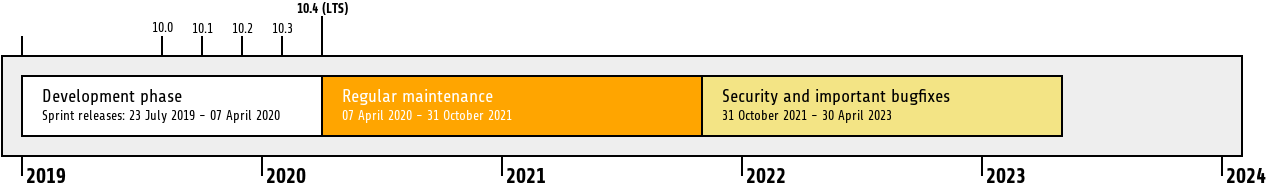
\includegraphics[width=1\linewidth]{Introduction/typo3-v10-lifecycle.png}
	\end{figure}

	\textbf{Erweiterter Support}\newline
	\smaller
		Die \href{https://typo3.com}{TYPO3 GmbH} bietet weitere Supportmöglichkeiten
		für TYPO3 v10 LTS auch nach dem 30. April 2023 für bis zu zwei weitere Jahre.
	\normalsize

\end{frame}

% ------------------------------------------------------------------------------
% TYPO3 v10 Roadmap

\begin{frame}[fragile]
	\frametitle{Einführung}
	\framesubtitle{TYPO3 v10 Roadmap}

	Veröffentlichungsdaten und ihr Hauptfokus:

	\begin{itemize}

		\item v10.0 \tabto{1.1cm}23/July/2019\tabto{3.4cm}Pave the way for exciting new concepts and APIs
		\item v10.1 \tabto{1.1cm}01/Oct/2019\tabto{3.4cm}Routing Improvements and Site Handling v2
		\item v10.2 \tabto{1.1cm}03/Dec/2019\tabto{3.4cm}Fluid/Rendering Engine Improvements
		\item
			\begingroup
				\color{typo3orange}
				v10.3 \tabto{1.1cm}25/Feb/2020\tabto{3.4cm}Feature Freeze
			\endgroup
		\item v10.4 \tabto{1.1cm}21/Apr/2020\tabto{3.4cm}LTS Release (Long-term Support)

	\end{itemize}

	\vspace{0.6cm}
	\smaller
		\url{https://typo3.org/article/typo3-v10-roadmap/}\newline
		\url{https://typo3.org/article/typo3-v10-safe-and-sound/}
	\normalsize

\end{frame}

% ------------------------------------------------------------------------------
% Installation

\begin{frame}[fragile]
	\frametitle{Einführung}
	\framesubtitle{Installation}

	\begin{itemize}
		\item Empfohlene \textit{klassische} Installationsschritte unter Linux/Mac OS X\newline
			(DocumentRoot ist beispielweise \texttt{/var/www/site/htdocs}):
\begin{lstlisting}
$ cd /var/www/site
$ wget --content-disposition get.typo3.org/10.3
$ tar xzf typo3_src-10.3.0.tar.gz
$ cd htdocs
$ ln -s ../typo3_src-10.3.0 typo3_src
$ ln -s typo3_src/index.php
$ ln -s typo3_src/typo3
$ touch FIRST_INSTALL
\end{lstlisting}

		\item Symbolische Links unter Microsoft Windows:

			\begin{itemize}
				\item Unter Windows XP/2000 kann \texttt{junction} benutzt werden
				\item Unter Windows Vista und Windows 7 oder höher kann \texttt{mklink} benutzt werden
			\end{itemize}

	\end{itemize}
\end{frame}

% ------------------------------------------------------------------------------
% Installation using composer

\begin{frame}[fragile]
	\frametitle{Installation and Upgrade}
	\framesubtitle{Installation mit \texttt{composer}}

	\begin{itemize}
		\item Installation mit \textit{composer} unter Linux, Mac OS X und Windows 10:
\begin{lstlisting}
$ cd /var/www/site/
$ composer create-project typo3/cms-base-distribution typo3v10 ^10.3
\end{lstlisting}

		\item Alternativ eine benutzerdefinierte \texttt{composer.json} Datei erstellen und ausführen:
\begin{lstlisting}
$ composer install
\end{lstlisting}

			Weitere \texttt{composer.json} Beispieldateien befinden sich unter\newline
			\smaller
				\href{https://composer.typo3.org}{https://composer.typo3.org}.
			\normalsize

	\end{itemize}
\end{frame}

% ------------------------------------------------------------------------------
